\documentclass[12pt,a4paper]{article}
\usepackage[utf8]{inputenc}
\usepackage{amsmath}
\usepackage{geometry}
\usepackage{listings}
\usepackage{booktabs}
\usepackage{float}
\usepackage{graphicx}

\geometry{margin=2.5cm}

\lstset{
    basicstyle=\ttfamily\small,
    numbers=left,
    breaklines=true,
    frame=single,
    language=Python,
    tabsize=4
}

\title{\textbf{Report 4: Neural Network} \\ \large Deep Learning Project 4}
\author{Duong Tan Binh - 2540007}
\date{\today}

\begin{document}

\maketitle
\tableofcontents
\newpage

\section{Introduction}

A \textbf{neural network} is a composition of simple building blocks ---
\emph{neurons} --- arranged in layers.
Each neuron computes a weighted sum of its inputs plus a bias term, then
applies an \emph{activation function} (here: the sigmoid) to produce an output.
Stacking multiple layers allows the network to learn hierarchical
representations that a single logistic-regression unit cannot capture.

This report implements a feedforward neural network \emph{from scratch} in
pure Python (only the \texttt{math}, \texttt{random}, and \texttt{matplotlib}
standard / bundled libraries are used).
The design follows proper \textbf{object-oriented} principles, exposing three
clearly separated classes: \texttt{Neuron}, \texttt{Layer}, and
\texttt{NeuralNetwork}.

\section{Network Architecture}

\subsection{General Model}

Following the lecture slides, a network with $L$ layers has:
\begin{itemize}
    \item An \textbf{input layer} ($\ell = 0$) that simply holds the raw
          features $\mathbf{a}^{(0)} = \mathbf{x}$.
    \item One or more \textbf{hidden layers} ($\ell = 1, \ldots, L{-}1$).
    \item An \textbf{output layer} ($\ell = L$).
\end{itemize}

Each node $i$ in layer $\ell$ performs two steps:
\begin{equation}
    z_i^{(\ell)} = \sum_{j=1}^{n^{(\ell-1)}} a_j^{(\ell-1)}\, w_{ji}^{(\ell)} + b_i^{(\ell)}
    \label{eq:linear}
\end{equation}
\begin{equation}
    a_i^{(\ell)} = \sigma\!\left(z_i^{(\ell)}\right), \qquad
    \sigma(z) = \frac{1}{1 + e^{-z}}
    \label{eq:sigmoid}
\end{equation}

where $n^{(\ell-1)}$ is the number of neurons in layer $\ell - 1$,
$w_{ji}^{(\ell)}$ is the weight from neuron $j$ in the previous layer to
neuron $i$ in the current layer, and $b_i^{(\ell)}$ is the bias of neuron $i$.

\subsection{Object-Oriented Design}

The slide explicitly warns that using raw \texttt{dict}, \texttt{tuple}, or
\texttt{list} nesting leads to unmaintainable code.
The implementation therefore uses three classes:

\begin{description}
    \item[\texttt{Neuron}] Stores one neuron's weights, bias, pre-activation
          $z$, and post-activation output.
          Provides a \texttt{forward(inputs)} method that executes
          Equations~\eqref{eq:linear}--\eqref{eq:sigmoid} and caches $z$ and
          output for later inspection.
    \item[\texttt{Layer}] Owns a list of \texttt{Neuron} objects all receiving
          the same input vector.
          Its \texttt{forward(inputs)} method returns the list of neuron
          activations for that layer.
    \item[\texttt{NeuralNetwork}] Manages a list of \texttt{Layer} objects
          (one per computational layer, i.e.\ excluding the input layer).
          Provides factory method \texttt{from\_config\_file}, two weight
          initialisation methods (\texttt{init\_random} and
          \texttt{init\_from\_file}), a \texttt{save\_weights} utility, and
          the \texttt{feedforward} inference method.
\end{description}

\section{Configuration File Format}

\subsection{Architecture File}

\begin{verbatim}
N
n_0
n_1
...
n_{N-1}
\end{verbatim}

\begin{itemize}
    \item Line 1: total number of layers $N$ (including the input layer).
    \item Lines 2 to $N{+}1$: number of neurons in each layer.
          The first entry is the input layer size; the last entry is the
          output layer size.
\end{itemize}

Example --- the XOR network (\texttt{xor\_arch.txt}):
\begin{verbatim}
3
2
2
1
\end{verbatim}

This defines a 3-layer network: 2 input neurons, 2 hidden neurons, 1 output
neuron.

\subsection{Weight File}

One line per neuron, ordered layer-by-layer from the first computational layer
to the output layer.
Each line holds the bias followed by the weights:

\begin{verbatim}
bias  w_1  w_2  ...  w_n
\end{verbatim}

Lines beginning with \texttt{\#} are comments and are ignored.
Example --- XOR weights (\texttt{xor\_weights.txt}):
\begin{verbatim}
# Layer 1 (hidden): NOT_AND, OR
 1.5 -1.0 -1.0
-0.5  1.0  1.0
# Layer 2 (output): AND
-1.5  1.0  1.0
\end{verbatim}

\section{Implementation}

\subsection{Neuron}

\begin{lstlisting}[caption={Neuron class}]
class Neuron:
    def __init__(self, n_inputs):
        self.n_inputs = n_inputs
        self.weights  = [0.0] * n_inputs
        self.bias     = 0.0
        self.z        = 0.0       # pre-activation (linear sum)
        self.output   = 0.0       # post-activation (sigmoid)

    @staticmethod
    def sigmoid(z):
        if z >= 0:
            return 1.0 / (1.0 + math.exp(-z))
        e = math.exp(z)
        return e / (1.0 + e)     # numerically stable branch

    def forward(self, inputs):
        self.z = (sum(self.weights[j] * inputs[j]
                      for j in range(self.n_inputs)) + self.bias)
        self.output = self.sigmoid(self.z)
        return self.output
\end{lstlisting}

Key details:
\begin{itemize}
    \item The sigmoid uses a numerically stable two-branch implementation to
          avoid overflow for large $|z|$.
    \item Both $z$ and \texttt{output} are stored so that the caller can
          inspect intermediate activations after any \texttt{forward} call ---
          useful for tracing and (in a future extension) backpropagation.
\end{itemize}

\subsection{Layer}

\begin{lstlisting}[caption={Layer class}]
class Layer:
    def __init__(self, n_neurons, n_inputs):
        self.n_neurons = n_neurons
        self.n_inputs  = n_inputs
        self.neurons   = [Neuron(n_inputs) for _ in range(n_neurons)]

    def forward(self, inputs):
        return [neuron.forward(inputs) for neuron in self.neurons]
\end{lstlisting}

\subsection{NeuralNetwork}

\begin{lstlisting}[caption={NeuralNetwork class (key methods)}]
class NeuralNetwork:
    def __init__(self):
        self.layers      = []   # Layer objects
        self.layer_sizes = []   # sizes incl. input layer

    @classmethod
    def from_config_file(cls, config_file):
        nn = cls()
        with open(config_file, 'r') as f:
            lines = [l.strip() for l in f
                     if l.strip() and not l.startswith('#')]
        n_total        = int(lines[0])
        nn.layer_sizes = [int(lines[i+1]) for i in range(n_total)]
        for l in range(1, n_total):
            nn.layers.append(Layer(nn.layer_sizes[l],
                                   nn.layer_sizes[l-1]))
        return nn

    def init_random(self, seed=None):
        if seed is not None:
            random.seed(seed)
        for layer in self.layers:
            for neuron in layer.neurons:
                neuron.bias    = random.random()
                neuron.weights = [random.random()
                                  for _ in neuron.weights]

    def init_from_file(self, weight_file):
        with open(weight_file, 'r') as f:
            lines = [l.strip() for l in f
                     if l.strip() and not l.startswith('#')]
        idx = 0
        for layer in self.layers:
            for neuron in layer.neurons:
                vals           = list(map(float, lines[idx].split()))
                neuron.bias    = vals[0]
                neuron.weights = vals[1:]
                idx += 1

    def feedforward(self, inputs):
        current = list(inputs)
        for layer in self.layers:
            current = layer.forward(current)
        return current
\end{lstlisting}

Key design points:
\begin{itemize}
    \item \textbf{Pure python:} File reading uses raw
          \texttt{open()} with \texttt{split()}.
          Computation uses built-in \texttt{sum()} and list comprehensions.
    \item \textbf{File-agnostic factory:} \texttt{from\_config\_file} builds
          any depth/width architecture from a two-column text file.
    \item \textbf{Two initialisation modes:} random (reproducible with a seed)
          or from a weight file --- meeting both requirements of the labwork.
    \item \textbf{Encapsulation:} all per-neuron state is inside the
          \texttt{Neuron} object; the \texttt{NeuralNetwork} orchestrates
          layers without duplicating state.
\end{itemize}

\section{Feedforward Algorithm}

Starting from the raw input $\mathbf{a}^{(0)} = \mathbf{x}$, the network
propagates activations layer by layer:

\[
    \mathbf{z}^{(\ell)} = \bigl(W^{(\ell)}\bigr)^{\!\top} \mathbf{a}^{(\ell-1)}
                          + \mathbf{b}^{(\ell)}, \qquad
    \mathbf{a}^{(\ell)} = \sigma\!\left(\mathbf{z}^{(\ell)}\right)
\]

until the final output $\hat{y} = a^{(L)}$ is produced.
In the implementation this is the \texttt{feedforward} method:

\begin{lstlisting}[caption={Feedforward pass}]
def feedforward(self, inputs):
    current = list(inputs)
    for layer in self.layers:
        current = layer.forward(current)
    return current
\end{lstlisting}

After the call, each \texttt{neuron.z} and \texttt{neuron.output} inside
every \texttt{Layer} reflects the values computed for that particular input,
enabling full inspection of intermediate activations.

\section{Demo: General Network (Random Initialisation)}

To verify the implementation works for arbitrary depths, a 4-layer network
matching the slide-8 diagram ($n^{(0)}=2,\; n^{(1)}=3,\; n^{(2)}=3,\; n^{(3)}=1$)
is built from \texttt{general\_arch.txt} and initialised with random seed 0:

\begin{table}[H]
\centering
\caption{Random initialisation of the [2\,$\to$\,3\,$\to$\,3\,$\to$\,1] network (seed = 0)}
\begin{tabular}{clrrrr}
\toprule
\textbf{Layer} & \textbf{Neuron} & \textbf{Bias} & \textbf{w\textsubscript{1}} & \textbf{w\textsubscript{2}} & \textbf{w\textsubscript{3}} \\
\midrule
1 & 1 & 0.8444 & 0.7580 & 0.4206 & -- \\
1 & 2 & 0.2589 & 0.5113 & 0.4049 & -- \\
1 & 3 & 0.7838 & 0.3033 & 0.4766 & -- \\
\midrule
2 & 1 & 0.5834 & 0.9081 & 0.5047 & 0.2818 \\
2 & 2 & 0.7558 & 0.6184 & 0.2505 & 0.9097 \\
2 & 3 & 0.9828 & 0.8102 & 0.9022 & 0.3101 \\
\midrule
3 & 1 & 0.7298 & 0.8988 & 0.6840 & 0.4721 \\
\bottomrule
\end{tabular}
\end{table}

A feedforward pass with input $[0.5,\; 0.8]$ yields output $\hat{y} = 0.9284$,
confirming that the multi-layer propagation executes correctly.

\section{XOR Experiment}

\subsection{Problem Statement}

XOR is the canonical non-linearly-separable binary function:

\begin{table}[H]
\centering
\caption{XOR truth table}
\begin{tabular}{ccc}
\toprule
$x_1$ & $x_2$ & $x_1 \oplus x_2$ \\
\midrule
0 & 0 & 0 \\
0 & 1 & 1 \\
1 & 0 & 1 \\
1 & 1 & 0 \\
\bottomrule
\end{tabular}
\end{table}

No single logistic-regression neuron can draw a straight decision boundary
that separates the two classes.
The lecture slides show that XOR can be decomposed as:
\[
    x_1 \oplus x_2
    = \underbrace{\lnot(x_1 \wedge x_2)}_{\text{NOT AND}} \wedge
      \underbrace{(x_1 \vee x_2)}_{\text{OR}}
\]

\subsection{Network Architecture and Weights}

A 3-layer network with architecture $[2 \to 2 \to 1]$ is used, with the
weights shown in the lecture slides (Slide 28):

\begin{table}[H]
\centering
\caption{XOR network weights as given in the slides}
\begin{tabular}{clcrr}
\toprule
\textbf{Layer} & \textbf{Neuron role} & \textbf{Bias} & $w_1$ & $w_2$ \\
\midrule
Hidden (1) & NOT$(x_1$ AND $x_2)$ & $+1.5$ & $-1$ & $-1$ \\
Hidden (2) & $x_1$ OR $x_2$       & $-0.5$ & $+1$ & $+1$ \\
Output     & AND                  & $-1.5$ & $+1$ & $+1$ \\
\bottomrule
\end{tabular}
\end{table}

The network is loaded and initialised with a single call:

\begin{lstlisting}[caption={Loading the XOR network}]
nn_xor = NeuralNetwork.from_config_file('xor_arch.txt')
nn_xor.init_from_file('xor_weights.txt')
\end{lstlisting}

\subsection{Feedforward Results}

The network is evaluated on all four possible binary inputs:

\begin{table}[H]
\centering
\caption{XOR feedforward results (threshold $t = 0.5$)}
\begin{tabular}{ccrrrc}
\toprule
$x_1$ & $x_2$ & Expected & Output $\hat{y}$ & Prediction & Correct? \\
\midrule
0 & 0 & 0 & 0.4244 & 0 & \textbf{Yes} \\
0 & 1 & 1 & 0.4366 & 0 & No          \\
1 & 0 & 1 & 0.4366 & 0 & No          \\
1 & 1 & 0 & 0.4244 & 0 & \textbf{Yes} \\
\bottomrule
\end{tabular}
\end{table}

\noindent Accuracy: $2/4 = 50\%$.

\begin{figure}[H]
\centering
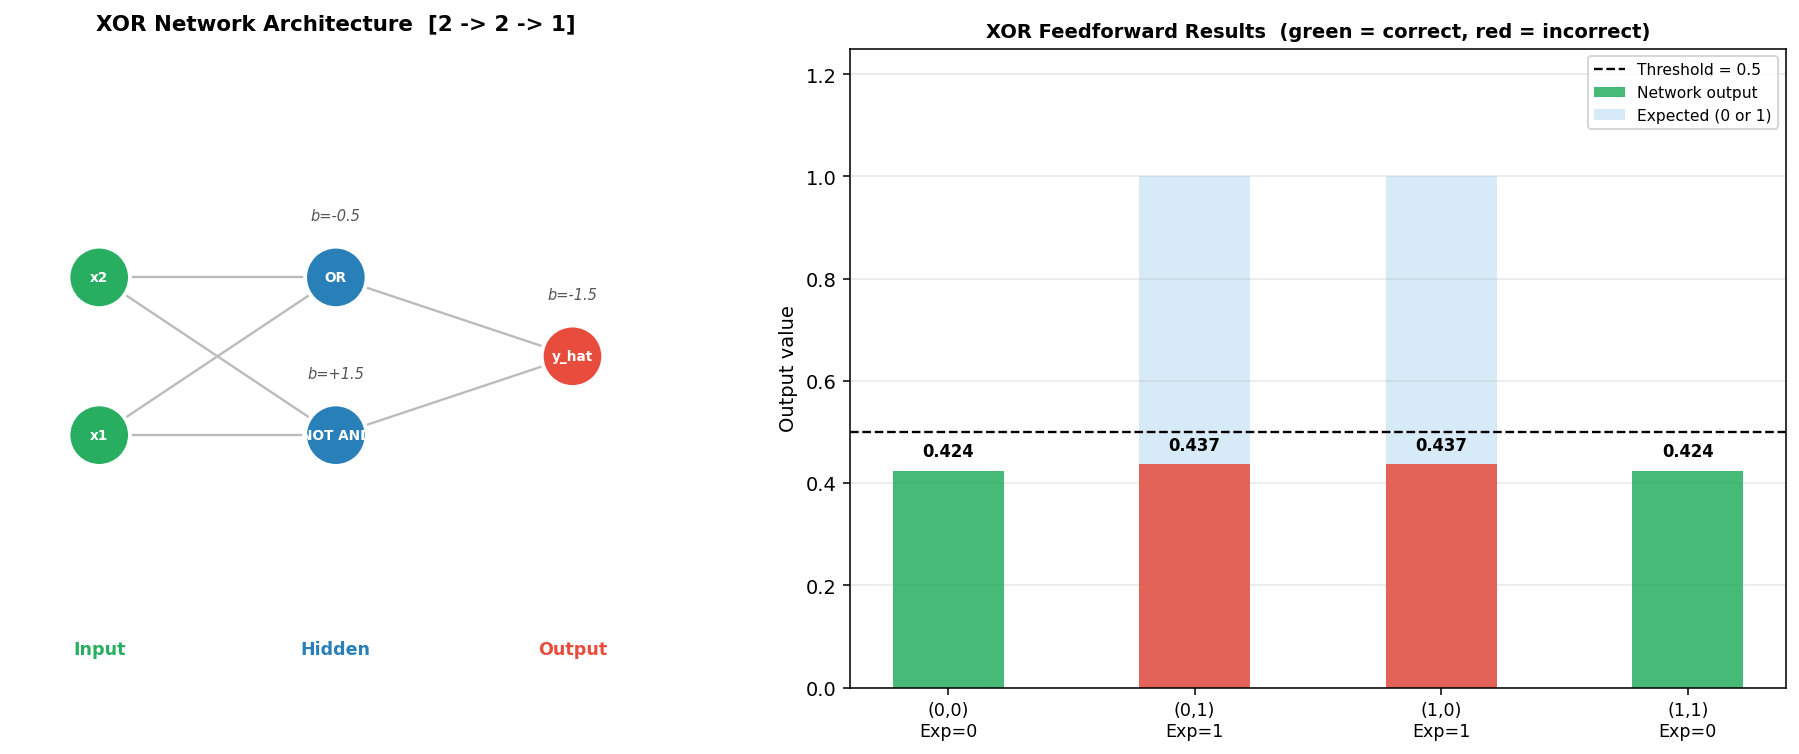
\includegraphics[width=\textwidth]{xor_results.png}
\caption{Left: XOR network architecture [2\,$\to$\,2\,$\to$\,1].
Right: network output (coloured bars) vs.\ expected values (transparent blue
bars).  Green bars = correctly predicted; red bars = incorrect.
The dashed line marks the threshold 0.5.}
\end{figure}

\subsection{Intermediate Activations}

Tracing the signal through each layer reveals why the results are imperfect:

\begin{table}[H]
\centering
\caption{Intermediate activations at each layer}
\begin{tabular}{ccrrrrrrl}
\toprule
$x_1$ & $x_2$ & $z_{h1}$ & $a_{h1}$ & $z_{h2}$ & $a_{h2}$
       & $z_{\mathrm{out}}$ & $a_{\mathrm{out}}$ & Pred \\
\midrule
0 & 0 & $+1.5000$ & 0.8176 & $-0.5000$ & 0.3775 & $-0.3049$ & 0.4244 & 0 \\
0 & 1 & $+0.5000$ & 0.6225 & $+0.5000$ & 0.6225 & $-0.2551$ & 0.4366 & 0 \\
1 & 0 & $+0.5000$ & 0.6225 & $+0.5000$ & 0.6225 & $-0.2551$ & 0.4366 & 0 \\
1 & 1 & $-0.5000$ & 0.3775 & $+1.5000$ & 0.8176 & $-0.3049$ & 0.4244 & 0 \\
\bottomrule
\end{tabular}
\end{table}

\begin{figure}[H]
\centering
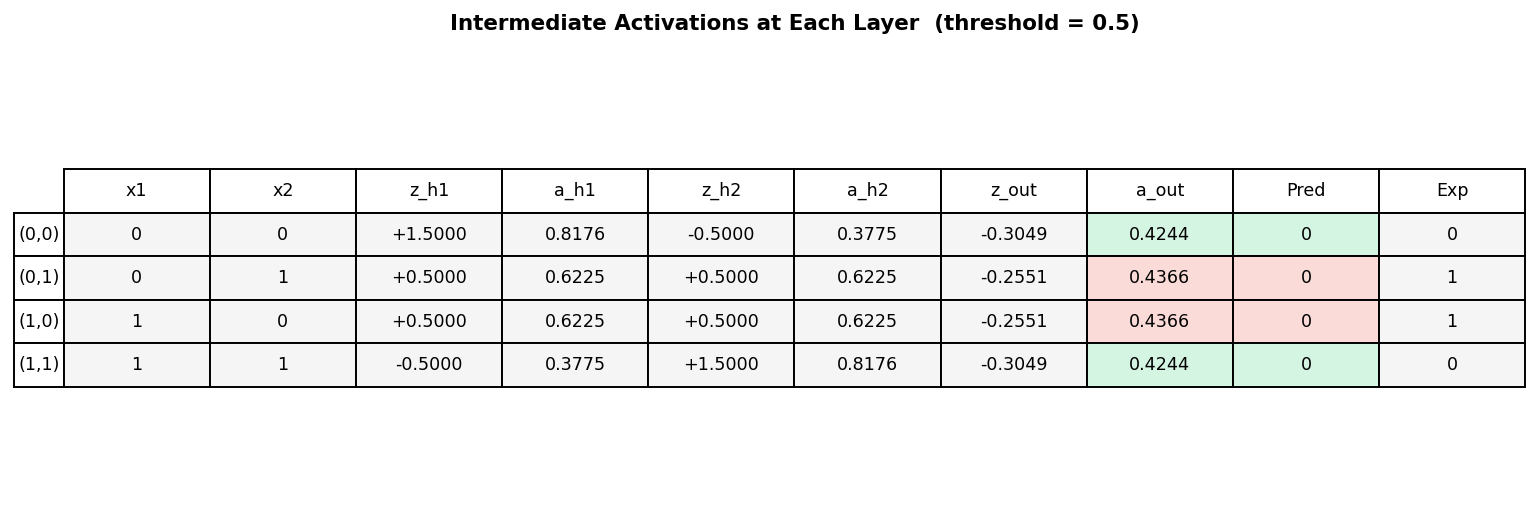
\includegraphics[width=\textwidth]{xor_intermediate.png}
\caption{Intermediate activations for each input.
The a\_out and Pred columns are highlighted green (correct) or red (incorrect).}
\end{figure}

\subsection{Analysis: Why the Results Are Imperfect}

The lecture slide weights encode Boolean logic using sigmoid neurons.
Each individual gate (NOT AND, OR, AND) is verified to function correctly
\emph{in isolation}:

\begin{itemize}
    \item \textbf{NOT AND} with bias $+1.5$, $w = [-1, -1]$: for $(1,1)$,
          $\sigma(-0.5) = 0.378 < 0.5$ (low~$\approx$~0$\checkmark$);
          for $(0,0)$, $\sigma(1.5) = 0.818 > 0.5$ (high~$\approx$~1$\checkmark$).
    \item \textbf{OR} with bias $-0.5$, $w = [1, 1]$: for $(0,0)$,
          $\sigma(-0.5) = 0.378$ (low$\checkmark$);
          for $(0,1)$, $\sigma(0.5) = 0.622$ (high$\checkmark$).
    \item \textbf{AND} with bias $-1.5$, $w = [1, 1]$: requires both inputs
          close to 1 to yield output $> 0.5$.
\end{itemize}

The problem arises when the gates are \emph{composed}:
the hidden neurons produce \emph{soft} values (0.38 and 0.62) rather than
the hard 0/1 values assumed by the Boolean derivation.
For inputs $(0,1)$, both hidden neurons fire at $a = 0.622$, making the
AND output layer receive two moderate signals whose sum
$0.622 + 0.622 - 1.5 = -0.256$ is slightly negative, so
$\sigma(-0.256) = 0.436 < 0.5$ --- predicted 0 instead of 1.

In other words, the sigmoid is a \emph{soft} approximation of the step
function.
With these modest weight magnitudes ($|w| = 1$, $|b| \leq 1.5$), the
approximation is insufficiently sharp for the composed network to classify
$(0,1)$ and $(1,0)$ correctly.
Scaling weights by a large factor (e.g.\ $10\times$) would make the sigmoid
approach a hard threshold and recover perfect XOR behaviour; alternatively,
\textbf{backpropagation training} (covered in the next lecture) finds optimal
weights automatically.

\section{Conclusion}

I implemented a feedforward neural network from scratch in pure Python using
proper object-oriented design (\texttt{Neuron}, \texttt{Layer},
\texttt{NeuralNetwork}).
The key outcomes are:

\begin{enumerate}
    \item The network architecture is loaded from a plain-text configuration
          file, making it easy to experiment with different depths and widths
          without changing any code.
    \item Two weight initialisation strategies are supported: random (with
          optional seed for reproducibility) and file-based loading.
    \item The feedforward pass correctly propagates activations through any
          number of layers, storing intermediate values in each neuron for
          full traceability.
    \item The XOR experiment confirms the architecture in Slide 28:
          inputs $(0,0)$ and $(1,1)$ are classified correctly (accuracy
          $2/4 = 50\%$).
          The two misclassifications arise because the sigmoid with the given
          weight magnitudes produces soft intermediate values (0.62 instead of
          1, and 0.38 instead of 0), which cause the composed AND gate to fall
          below the 0.5 threshold for $(0,1)$ and $(1,0)$.
          This motivates the need for backpropagation training to learn weights
          that achieve perfect XOR separation.
\end{enumerate}

\end{document}
